\chapter{Analyse et spécification des besoins}
\label{chap:analyse}

\section*{Introduction}
\addcontentsline{toc}{section}{Introduction}

Ce chapitre présente l'analyse des besoins qui a servi de base à la conception du système : identification des acteurs, formalisation des besoins fonctionnels et non fonctionnels, modélisation des cas d'utilisation, et constitution du backlog produit.

\section{Identification des acteurs}

L'étude de l'existant et les échanges avec l'encadrant professionnel ont permis d'identifier les acteurs suivants, humains et systèmes :

\begin{itemize}
    \item \textbf{Client e-commerce} : le visiteur ou acheteur du site marchand, qui interagit avec l'assistant conversationnel pour rechercher des produits, poser des questions ou demander un code promotionnel.
    \item \textbf{Administrateur} (marchand / tenant) : l'utilisateur du backoffice, responsable de la configuration du comportement de l'assistant, du suivi de son activité et du pilotage des actions d'administration.
    \item \textbf{Agent IA d'administration} : composant système déclenché par l'administrateur, exécutant un ensemble d'actions prédéfinies (analytique, génération de coupons, stratégie marketing) sous supervision.
    \item \textbf{PrestaShop} (acteur externe) : la plateforme e-commerce source du catalogue produits.
    \item \textbf{Fournisseur de modèle de langage} (Groq) : acteur externe sollicité pour la génération de réponses en langage naturel.
\end{itemize}

\section{Besoins fonctionnels}

Les besoins fonctionnels ont été regroupés par acteur principal.

\subsection{Côté client}

\begin{itemize}
    \item Poser une question en langage naturel et obtenir une réponse contextualisée par le catalogue produits du tenant.
    \item Rechercher un produit et obtenir des recommandations pertinentes (produits similaires, produits tendance).
    \item Obtenir, dans certains contextes définis par l'administrateur (ex. relance panier, fidélisation), un code promotionnel généré automatiquement.
    \item Voir sa demande traitée de façon fiable même lorsque le modèle de langage ne peut apporter de réponse pertinente (dégradation contrôlée plutôt qu'échec silencieux).
\end{itemize}

\subsection{Côté administrateur}

\begin{itemize}
    \item Consulter un tableau de bord présentant l'activité réelle du chat (volume de conversations, taux de reconnaissance d'intention, coût d'utilisation du modèle de langage, blocages de sécurité).
    \item Définir des \textbf{règles métier} (conditions sur l'intention détectée ou des mots-clés, associées à une action : réponse automatique, instruction injectée, génération de coupon), sans intervention technique.
    \item Interroger un \textbf{agent IA d'administration} en langage naturel ou via une action structurée, pour obtenir des statistiques, déclencher une génération de coupons en masse ou obtenir une suggestion de stratégie marketing.
    \item Confirmer, ou annuler, toute action d'administration à impact avant son exécution effective.
    \item Consulter les indicateurs de demande client réelle : produits les plus demandés, recherches infructueuses (signal de lacune du catalogue), répartition des intentions, heures de pointe, taux de conversion des coupons, produits en stock faible.
    \item Parcourir l'historique des conversations traitées par l'assistant.
    \item Suivre la consommation et le coût d'utilisation du modèle de langage sur une période donnée.
\end{itemize}

\section{Besoins non fonctionnels}

\begin{itemize}
    \item \textbf{Isolation multi-tenant} : chaque tenant ne doit avoir accès qu'à ses propres données (conversations, règles, produits) ; cette contrainte doit être appliquée de façon systématique au niveau de la couche d'accès aux données, non laissée à la discrétion de chaque endpoint.
    \item \textbf{Sécurité de l'exécution automatisée} : l'agent IA d'administration ne doit pouvoir exécuter qu'un ensemble fermé d'actions prédéfinies, chacune classée par niveau de risque, avec confirmation obligatoire au-delà d'un certain niveau.
    \item \textbf{Exactitude des données présentées} : toute métrique affichée dans le backoffice doit être calculée à partir de données réellement stockées ; à défaut de donnée source, la fonctionnalité doit l'indiquer explicitely plutôt que d'afficher une valeur inventée.
    \item \textbf{Traçabilité} : toute action d'administration exécutée doit être journalisée et consultable a posteriori.
    \item \textbf{Résilience} : la persistance d'un message, l'application d'une règle ou la génération d'un coupon ne doivent pas faire échouer la réponse au client en cas d'indisponibilité ponctuelle d'un composant secondaire (dégradation \emph{best-effort}).
    \item \textbf{Testabilité} : chaque fonctionnalité livrée doit être couverte par des tests automatisés reproductibles, exécutables en intégration continue.
\end{itemize}

\section{Diagramme de cas d'utilisation}

Le diagramme de la \cref{fig:usecase} synthétise les cas d'utilisation identifiés, organisés en trois sous-systèmes : les interactions côté client, la gestion administrative, et les intégrations externes (synchronisation du catalogue, indexation vectorielle). Le cas d'utilisation \emph{Configurer l'agent IA} y est réalisé, dans l'implémentation finale, par le module de gestion des règles métier détaillé au \cref{chap:conception}.

\begin{figure}[h]
    \centering
    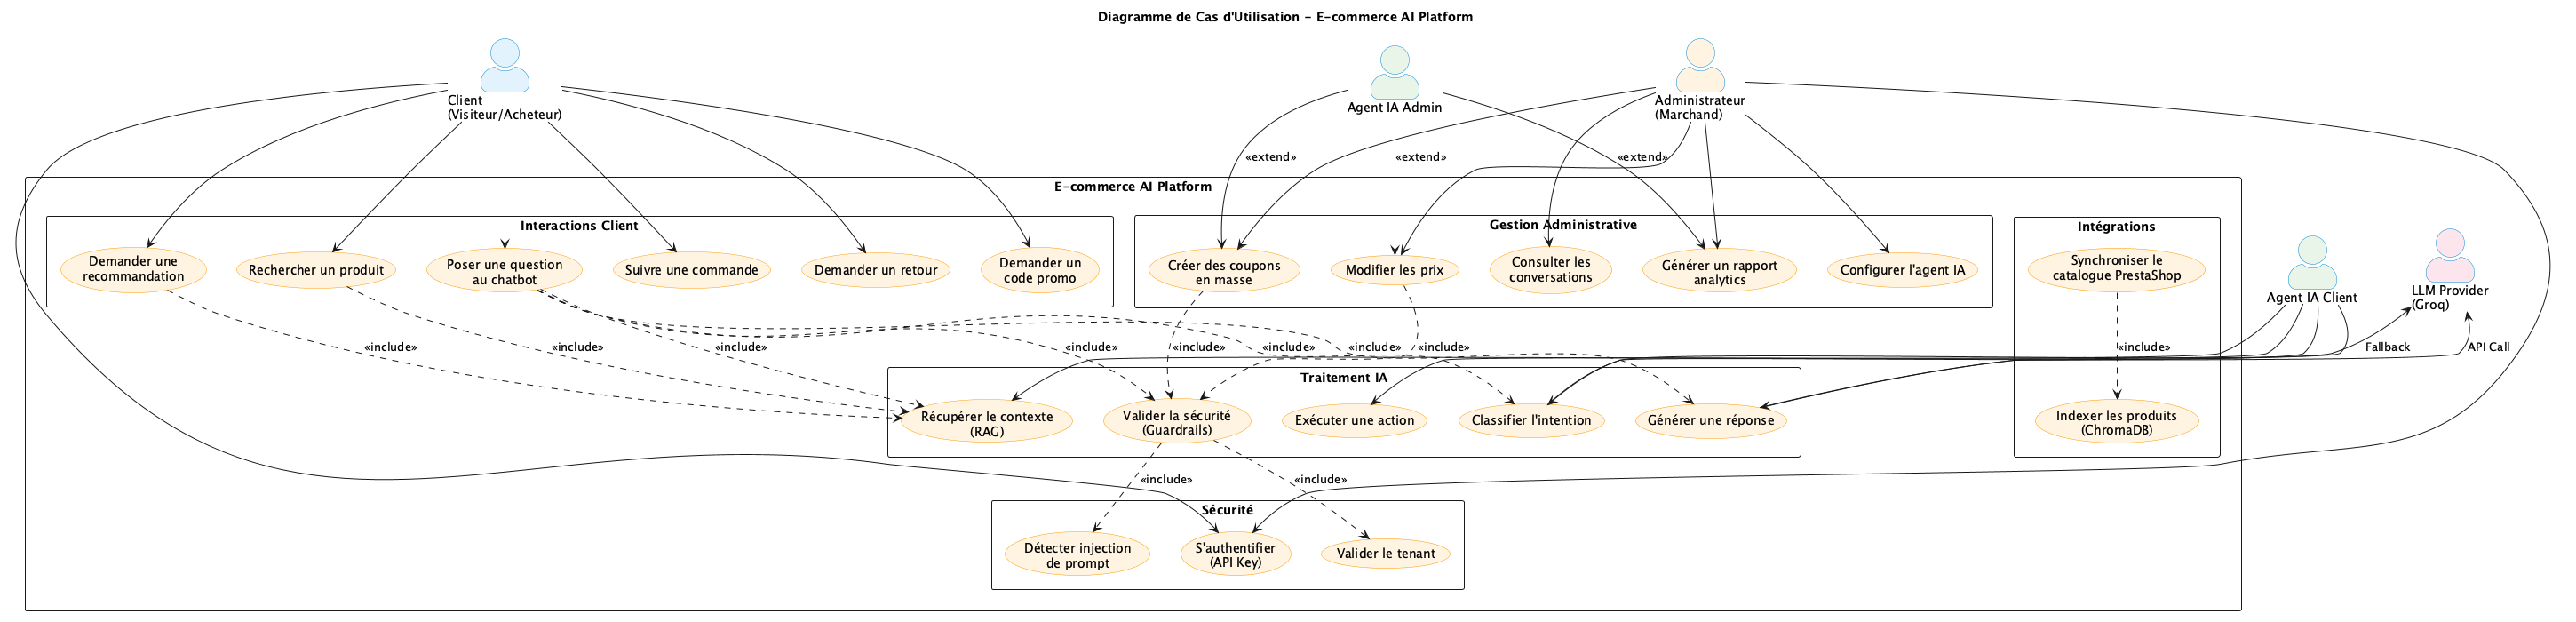
\includegraphics[width=\textwidth]{../diagrams/UseCase_Ecommerce_AI_Platform.png}
    \caption{Diagramme de cas d'utilisation de la plateforme}
    \label{fig:usecase}
\end{figure}

\section{Backlog produit}

Le \cref{tab:backlog} présente le backlog produit constitué à l'issue de la phase d'analyse, exprimé sous forme d'\emph{epics}. Chaque \emph{epic} a été décomposée en \emph{user stories} au moment de la planification du sprint correspondant (voir \cref{chap:realisation}).

\begin{table}[h]
\centering
\caption{Backlog produit (epics, par ordre de priorité)}
\label{tab:backlog}
\begin{tabular}{@{}p{0.5cm}p{6cm}p{6.5cm}@{}}
\toprule
\textbf{\#} & \textbf{Epic} & \textbf{Valeur métier} \\
\midrule
1 & Fondations techniques (infrastructure, modèles de données, synchronisation catalogue) & Prérequis à toute fonctionnalité \\
2 & Chat conversationnel augmenté (RAG) & C\oe{}ur de la proposition de valeur produit \\
3 & Sécurité, multi-tenance et supervision & Condition de mise en production \\
4 & Backoffice -- socle (tableau de bord, agent IA -- première version) & Autonomie de l'administrateur \\
5 & Moteur de règles métier \& agent IA d'administration sécurisé & Personnalisation sans intervention technique \\
6 & Analytique réelle \& finalisation backoffice & Confiance dans les données présentées \\
\bottomrule
\end{tabular}
\end{table}

\section*{Conclusion}
\addcontentsline{toc}{section}{Conclusion}

L'analyse menée dans ce chapitre a permis de traduire la problématique du stage en besoins concrets, priorisés sous forme de backlog. Le chapitre suivant détaille la conception technique retenue pour répondre à ces besoins.
